\documentclass[a4paper,10pt,titlepage]{article}
% PREUMBULUM
\usepackage[utf8]{inputenc}
\usepackage[T1]{fontenc}

\usepackage{a4wide} 
\usepackage{times}

\usepackage[magyar,english]{babel}

% Tartalomjegyzék:
\usepackage{tocbibind}

\usepackage[usenames,dvipsnames]{color}

% Hogy legyen képünk:
\usepackage{graphicx}

\usepackage{hyperref}
\hypersetup{
    bookmarks=true,
    unicode=true,
    colorlinks=true,
    linkcolor=RoyalBlue,
    citecolor=RoyalBlue,
    filecolor=RoyalBlue,
    urlcolor=RoyalBlue,
}

% Táblázatoknak:
\usepackage{colortbl}

\begin{document}
% Dokumentumtörzs

\selectlanguage{magyar}

\begin{titlepage}
\title{Hallgatói segédlet a jelentkezes.tnt.bme.hu oldal használatához}
\author{Nádudvari György \\
\texttt{ulqp9p csavaroskukac gmail pont com}}
\date{\today}
\end{titlepage}
\maketitle

\section{Bevezetés}

A BME Testnevelési Központ a 2011/12. tavaszi félévben új jelentkező felületet vezetett be azzal a szándékkal, hogy a gyűjtő kurzusokat felvett hallgatók életét megkönnyítse. Az első visszajelzések alapján ez nem feltétlenül sikerült, mivel sokatok problémákkal találkozott a \href{https://jelentkezes.tnt.bme.hu}{https://jelentkezes.tnt.bme.hu} oldal használatával, főleg a regisztrációval kapcsolatban, ezért készült ez a kis leírás.

\section{Első (ajánlott) lépés}

Ha úgy érzed, hogy ismered a HSZK ural2-es szolgáltatásait, az ahhoz kapcsolódó @hszk.bme.hu e-mail címet, és hozzá is férsz ehhez a fiókodhoz, akkor ezt a részt át is ugorhatod. Ha nem, akkor kérlek figyelmesen olvasd el a következő sorokat, mert enélkül nem fogsz tudni jelentkezni sportágakra, kurzusokra.

\subsection{A HSZK-s account adminisztációs oldal használata}

Ebben a részben szigorúan csak a minket érintő dolgokra térnék ki. Először is lépj be a \href{https://accadmin.hszk.bme.hu/}{https://accadmin.hszk.bme.hu/} oldalra a neptunkódoddal és neptunos jelszavaddal (\ref{fig:hszk_acc_admin_login}. ábra). Ne felejtsd el a felhasználói szabályzattal kapcsolatos pipát!

\begin{figure}[h!]
\centering
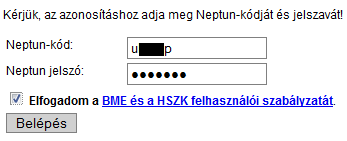
\includegraphics[width=0.50\textwidth]{figures/hszk_acc_admin_login.png}
\caption{Bejelentkezés a HSZK-s adminisztrációs oldalra \label{fig:hszk_acc_admin_login}}
\end{figure}

Sikeres bejelentkezés után keresd meg a \textit{HSZK Ural2 szerver használata} részt. Itt a második oszlopban találod a saját e-mailcímed felhasználói nevét (a kukac/@ előtti rész) (\ref{fig:hszk_acc_admin_mailcim}. ábra).

\begin{figure}[h!]
\centering
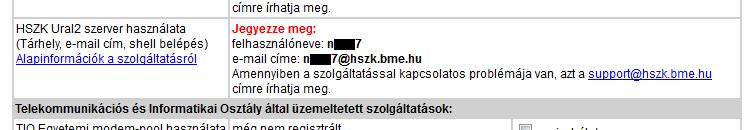
\includegraphics[width=0.80\textwidth]{figures/hszk_acc_admin_mailcim.png}
\caption{A HSZK-s emailcímed \label{fig:hszk_acc_admin_mailcim}}
\end{figure}

Ezután az oldal alján keresd meg a jelszó beállításával kapcsolatos részt (\ref{fig:hszk_acc_admin_jelszo}. ábra). Itt adjál meg egy tetszőleges, a kívánt szabályoknak megfelelő jelszót, kattints a \textit{Fenti módosítások érvényesítése}, majd a \textit{Kilépés} gombra.

\begin{figure}[h!]
\centering
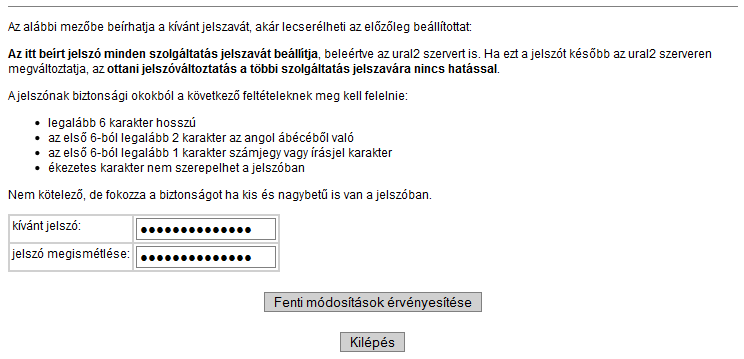
\includegraphics[width=0.80\textwidth]{figures/hszk_acc_admin_jelszo.png}
\caption{Jelszó beállítása \label{fig:hszk_acc_admin_jelszo}}
\end{figure}

\end{document}